\subsection{Công nghệ lưu trữ - PostgreSQL}

\subsubsection{Tổng quan về PostgreSQL}
PostgreSQL, còn được gọi là Postgres, là một hệ thống quản lý cơ sở 
dữ liệu quan hệ miễn phí mã nguồn mở chú trọng vào tính mở rộng và 
tính tương thích với chuẩn SQL. Ban đầu có tên là POSTGRES, có nguồn
gốc từ cơ sở dữ liệu Ingress được phát triển tại

Đại học California, Berkeley. Vào năm 1996, dự án được đổi tên thành
PostgreSQL. PostgreSQL được viết bằng ngôn ngữ C và có thể chạy trên nhiều
hệ điều hành như Linux, macOS, Windows, \ldots Đồng thời hỗ trợ các tính
năng tương tự như nhiều các cơ sở dữ liệu quan hệ khác.
Phiên bản PostgreSQL sử dụng trong đồ án này là 11.8.

\subsubsection{Tổng quan về Index}
Index trong cơ sở dữ liệu là một cấu trúc dữ liệu giúp cải thiện
tốc độ truy vấn dữ liệu trên các bảng với đánh đổi là sử dụng thêm
không gian lưu trữ nhằm duy trì cấu trúc dữ liệu index cũng như
làm tăng thời gian ghi dữ liệu. Index được sử dụng để nhanh chóng
định vị dữ liệu mà không phải tìm duyệt qua toàn bộ các hàng trong
bảng của cơ sở dữ liệu mỗi khi bảng đó được truy cập. Index có thể
được tạo sử dụng một hay nhiều cột trong cùng một bảng, cung cấp
cơ chế tăng tốc quá trình tra cứu ngẫu nhiên và truy cập có thứ
tự các bản ghi trong cơ sở dữ liệu. 

Index được chia làm hai loại kiến trúc:
Clustered Index và Non-clustered Index.

Với clustered index, các hàng trong cơ sở dữ liệu được lưu trữ
trên đĩa theo cùng thứ tự với index. Do đó mỗi bảng chỉ tồn tại
duy nhất một clustered index. Với non-clustered index thì cấu trúc dữ
liệu index là cấu trúc dữ liệu nằm ngoài bảng, các hàng trong bảng
không được đảm bảo thứ tự giống như thứ tự của index. Một bảng có
thể có rất nhiều non-clustered index. Thông thường với truy cập trên
clustered index sẽ nhanh hơn trên non-clustered index vì dữ liệu
sẽ không bị phân mảnh ở nhiều vị trí trong ổ cứng.

\subsubsection{Index trong PostgreSQL}
Trong PostgreSQL, clustered index không được hỗ trợ. Tuy nhiên
PostgreSQL lại hỗ trợ nhiều kiểu index như B-Tree, Hash, GiST,
SP-GiST, GIN và BRIN. Mỗi một kiểu index sử dụng một thuật toán
riêng biệt để tối ưu cho nhiều loại câu truy vấn khác nhau.
Mặc định khi sử dụng lệnh CREATE INDEX thì index B-Tree sẽ được tạo,
index này cũng phù hợp với hầu hết các
trường hợp truy vấn~\cite{postgresdocs:online}.

Index kiểu B-Tree có thể được xử dụng cho các câu truy vấn
liên quan đến tìm kiếm bằng, tìm kiếm khoảng hoặc trong trường
hợp dữ liệu được sắp xếp theo một trường nào đó. Trình lập kế hoạch
cho các truy vấn của PostgreSQL sẽ xem xét sử dụng index B-Tree
bất kì khi nào trường mà có index nằm trong một trong
các phép toán so sánh như $<$ $<=$ $=$ $>=$ $>$.

Các toán tử tương đương hoặc tổ hợp của chúng, như là phép toán
BETWEEN và IN, cũng có thể sử dụng được index B-Tree.
Ngoài ra các phép toán liên quan đến NULL như IS NULL hay
IS NOT NULL cũng có thể được tăng tốc bằng index B-Tree.

Trình tối ưu cũng có thể sử dụng index B-Tree cho các câu
truy vấn sử dụng toán tử pattern matching như LIKE và ~
nếu mà pattern được sử dụng bắt đầu là một xâu hằng số
như ‘foo\%’ nhưng không phải là ‘\%bar’. 

B-Tree có thể cũng được sử dụng để lấy dữ liệu được sắp
xếp theo thứ tự của cột được index.

Index kiểu Hash chỉ có thể được sử dụng trong các câu truy
vấn sử dụng toán tử so sánh bằng. Để tạo index Hash trong PostgreSQL,
ta sử dụng:
\begin{lstlisting}[caption={Tạo index sử dụng Hash}, captionpos=b]
CREATE INDEX name ON table USING HASH (column);
\end{lstlisting}

\subsubsection{Full Text Search trên PostgreSQL}
\paragraph{Cơ bản về Full Text Search}
Các toán tử tìm kiếm text trên các CSDL quan hệ đã tồn
tại từ rất lâu như LIKE hay ILIKE. Nhưng những toán tử đó thiếu
đi những tính chất mà cần có trong các hệ thống thông tin hiện đại như:
\begin{itemize}[topsep=0ex]
\item Hỗ trợ ngôn ngữ, thậm chí với cả tiếng Anh. Các toán tử
    trên không phù hợp cho việc xử lý những từ gần giống nghĩa hoặc
    được suy diễn, như satisfy và satisfies trong tiếng Anh. Có thể
    dùng toán tử logic OR để tìm kiếm cả 2 nhưng phải liệt kê rất
    nhiều trường hợp và một số từ có thể có rất nhiều từ
    được suy diễn hoặc gần nghĩa.

\item Không hỗ trợ xếp hạng (ranking) trên tập kết quả,
    dẫn đến tìm kiếm không hiệu quả khi mà có thể có tới rất
    nhiều document được tìm thấy trong một câu truy vấn.

\item Các phép toán đó thường chậm vì không hỗ trợ đánh chỉ
    số, mỗi một câu truy vấn phải duyệt qua toàn bộ các document.
\end{itemize}

PostgreSQL hỗ trợ tiền xử lý các document và đánh chỉ
số để tăng tốc các câu truy vấn. Tiền xử lý document bao gồm việc:
\begin{itemize}[topsep=0ex]
\item Phân tích document thành các token.
\item Chuyển các token thành các lexeme.
\item Lưu trữ các dữ liệu sau khi tiền xử lý
    document để tối ưu cho truy vấn.
\end{itemize}

Một document trong PostgeSQL thông thường là một cột chứa
xâu của bảng CSDL, hoặc có thể là một 
tổ hợp (thông qua phép ghép nối xâu) của những trường
đó trong một bảng hay trong nhiều bảng hoặc
có thể được truyền từ ngoài vào. 

Một token là một xâu biểu diễn một từ được phân tích ra từ document.

Một lexeme cũng là một xâu, tương tự như token, nhưng đã
được chuẩn hóa (normalize) sao cho những dạng khác nhau của
một từ trở thành giống nhau. Việc chuẩn hóa luôn luôn
thực hiện chuyển tất cả các kí tự thành lower-case, và thông
thường có cắt bỏ một vài các hậu tố như e hoặc es trong tiếng
Anh. Đồng thời ở bước chuyển từ token thành càng lexeme cũng
thông thường loại bỏ những stop word, là những từ rất phổ biến
trở thành vô nghĩa khi tìm kiếm, PostgreSQL sử dụng Dictionary
để thực thi bước này.

Dictionary trong PostgreSQL cho phép hiệu chỉnh quá trình
chuẩn hóa thành lexeme, bao gồm:
\begin{itemize}[topsep=0ex]
\item Định nghĩa các stop word được loại bỏ.
\item Ánh xạ các từ đồng nghĩa thành một từ.
\item Ánh xạ cụm từ thành một từ.
\item Ánh xạ các biến thể của một từ thành dạng chuẩn.
\end{itemize}

PostgreSQL sử dụng kiểu dữ liệu tsvector để lưu trữ dữ
liệu sau khi tiền xử lý document, đồng thời sử dụng kiểu
tsquery để biểu diễn các câu truy vấn.

Để chuyển từ một xâu sang kiểu tsvector ta sử dụng hàm
to\_tsvector. Còn để chuyển một xâu bất kì sang một tsquery,
ta sử dụng plainto\_tsquery. 

Để thực hiện Full Text Search một tsvector với một tsquery,
ta sử dụng toán tử @@.

\paragraph{Full Text Search cho tiếng Việt}
Để thực hiện Full Text Search với tiếng Việt,
trong đồ án này sử dụng một hàm được định nghĩa bằng SQL như sau: 
\begin{figure}[H]
\centering
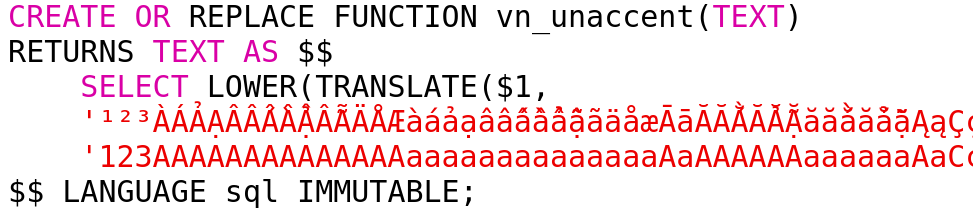
\includegraphics[width=10cm]{images/unaccent.png}
\end{figure}
Khi đó, thay vì sử dụng trực tiếp to\_tsvector và plainto\_tsquery,
ta sử dụng \\
to\_tsvector(vn\_unaccent(text)) và plainto\_tsquery(vn\_unaccent(text)).

\paragraph{Đánh chỉ số cho Full Text Search}
Để sử dụng Index cho Full Text Search, trước tiên ta cần tạo
một cột trong CSDL lưu trữ kiểu dữ liệu tsvector.
Có hai loại Index hay được sử dụng cho Full Text Search là GIN và GiST. 

\noindent Để Index sử dụng GIN, cú pháp như sau:
\begin{lstlisting}[caption={Tạo index sử dụng GIN},captionpos=b]
CREATE INDEX idx_textsearch ON sometable USING GIN (tsvector_column);
\end{lstlisting}

\noindent Còn nếu sử dụng GiST:
\begin{lstlisting}[caption={Tạo index sử dụng GiST},captionpos=b]
CREATE INDEX idx_textsearch ON sometable USING GIST (tsvector_column);
\end{lstlisting}

Khi đó toán tử @@ có thể sử dụng Index để
tăng tốc câu truy vấn. Trong PostgreSQL, Index Full Text Search
thông thường sử dụng GIN hơn sử dụng GiST. 

Thông thường sẽ sử dụng trigger để cập nhật các trường
tsvector trong CSDL khi chèn hoặc chỉnh sửa.

\paragraph{GIN}
\begin{figure}[H]
\centering
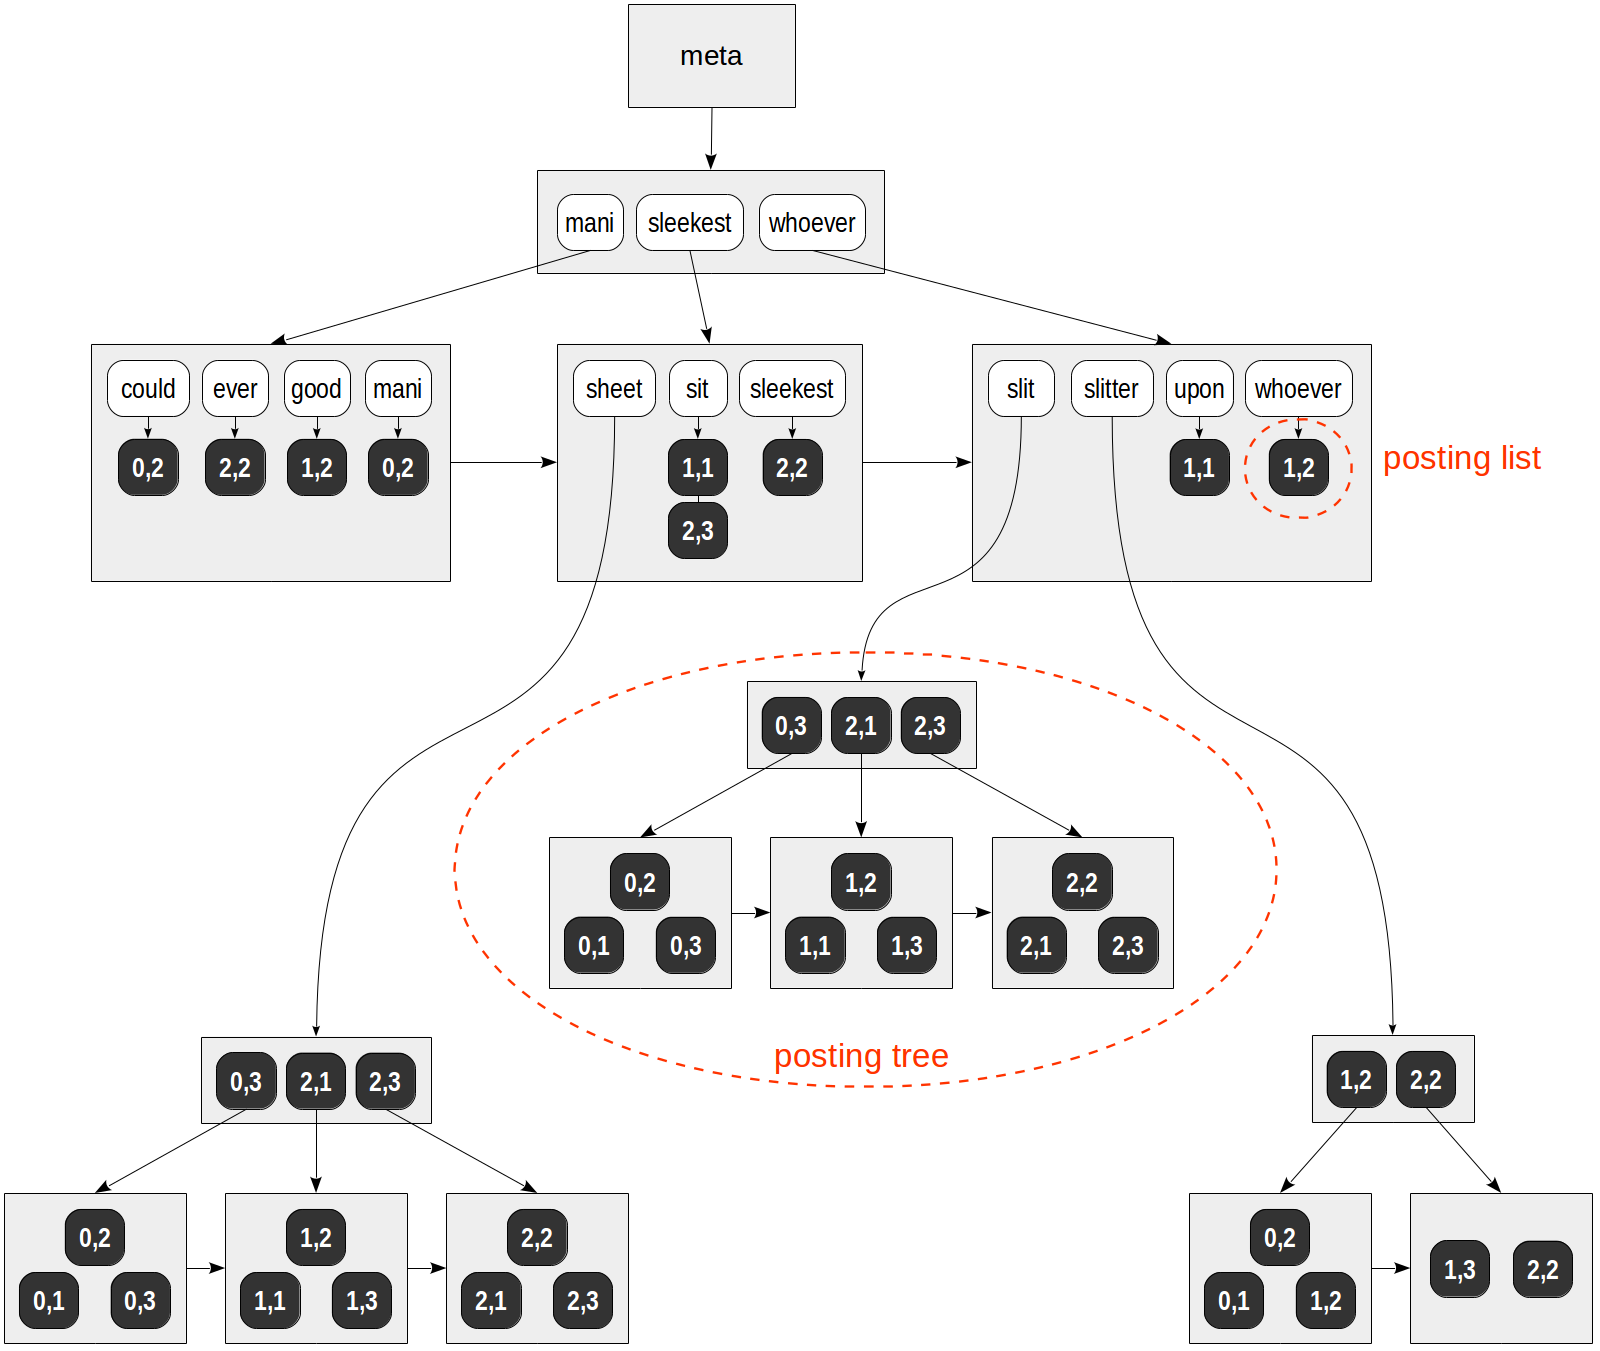
\includegraphics[width=13cm]{images/GIN.png}
\caption{Cấu trúc của GIN}
\end{figure}

GIN là viết tắt của Generalized Inverted Index. GIN được thiết
kế cho việc đánh chỉ số những giá trị tổng hợp (composite value),
và cho phép tìm kiếm cho các phần tử xuất hiện
trong các compostive value. 

Nếu quy ước một composite value là một item, còn phần tử trong
composite value là một key thì GIN 
luôn luôn lưu trữ và tìm kiếm trên key chứ không phải trên item.
Một GIN index lưu trữ tập các cặp (key, posting list) trong đó
posting list là tập các ID của các hàng trong bảng của CSDL.
Một ID có thể được nằm trong nhiều các posting list vì một
item có thể có nhiều các key. Mỗi một key được lưu trữ một
lần duy nhất, do đó nên GIN rất phù hợp trong trường hợp một
key xuất hiện nhiều lần. posting list được lưu với thứ tự
từ nhỏ đến lớn các ID của các hàng. Nếu posting list quá lớn
sẽ được chuyển thành posting tree, cấu trúc tương tự như B-Tree. 
